\documentclass[../main.tex]{subfiles}

\begin{document}

\section{Cathodes (Lucy/Hui/Arihant)}
\label{sec:cathodes}

\subsection{Introduction (Lucy)}
\label{sec:cathode_intro}
As mentioned in our introduction (sec~\ref{sec:intro}), lithium-ion batteries became promising materials in 1979 when Goodenough and Mizushima successfully showed LiCoO$_2$ as a cathode.\cite{mizushima1980lixcoo2} Since then, LIBs have become instrumental in electric vehicles and renewable energy grid storage applications \cite{rozier2015li,whittingham2008materials,dunn2011electrical, liu2013materials,palacin2009recent} to portable electronics such as mobile phones, which is largely attributed to their high energy density. \cite{masquelier2013polyanionic,armand2008building,bruce2012li,park2010review,scrosati2011lithium,goodenough_li-ion_2013,etacheri2011challenges,takada2013progress,fergus2010recent,ellis2010positive,he2012layered,zaghib2013review} For similar reasons, sodium-ion batteries have also gained increased attention, especially for grid storage applications. \cite{ellis2012curr,kim2012electrode,palomares2012ion,fergus2012ion,yabuuchi2012p2} Regardless of the application, the discovery of new materials and optimising current chemistries for improved performance is crucial for the next-generation of rechargeable batteries. With that in mind, it is known that the power density of the cathode material is the limiting factor in improving battery performance, thus many current research activities are focused on exploring cathode chemistries. These include layered oxides (Li\textit{M}O$_2$, \textit{M}=Co,Mn,Ni), spinel oxides (Li\textit{M}$_2$O$_4$), olivine phosphates (LiFePO$_4$), disordered rocksalts, lithium sulfur, and other compounds such as silicates. \cite{daniel2014cathode, islam2014lithium}

Layered transition metal oxides (Li\textit{M}O$_2$, \textit{M}=Co,Mn,Ni,etc.) are commonly considered as the first generation of cathode materials in commercial LIBs. Theses layered oxides possess a theoretical specific capacity of 270 mAh/g. However, their practical capacity is generally limited to below 200 mAh/g. \cite{myung2017nickel} LiCoO$_2$ held high capacities but the material was problematic due to capacity fading, low abundance, and the high cost of cobalt and ethical concerns surrounding geopolitical issues, making large scale applications impractical. \cite{mo2018impact} There is also considerable instability in LiCoO$_2$ structure, caused by the extraction of Li during cycling, which results in undesirable phase transitions from O3-type to O6-type Li$_x$CoO$_2$ and O1-type CoO$_2$. \cite{goonetilleke2018structural,chen2002staging} Other layered oxides also pose their own challenges, such as Li$_x$NiO$_2$ presenting capacity fade and poor safety, \cite{min2016comparative} and Li$_x$Mn$_2$O$_4$ presenting low capacity. \cite{tian2018performance} An emerging alternative to solve some of these challenges is using a combination of the transition metals. In 2000 \citeauthor{paulsen2000o2} presented Li$_{2/3}$[Ni$_{1/3}$Mn$_{2/3}$]O$_2$, \cite{paulsen2000o2,paulsen20002} with Li[Ni$_x$Mn$_{1-2x}$Co$_z$]O$_2$ (NMC) presented by the authors in 2001. \cite{lu2001layered} Partially replacing Co in LiCoO$_2$ with Ni and Mn to obtain layered Li[Ni$_x$Mn$_y$Co$_z$]O$_2$, \cite{rozier2015li} where $x+y+z=1$, shows improved electrochemical performance while also reducing material cost and improving stability.\cite{ohzuku2001layered} These layered oxides are commonly termed as NMC, with the subsequent numbering relating to the ratio between the cations.

A huge benefit of combining these transition metals is the ability to tune the transition metal composition to optimise aspects including capacity, cyclic rate, electrochemical stability, and lifetime, with the potential of reaching capacities $>220$ mAh g$^{-1}$. \cite{duan2019insights} Some NMC compositions are already used commercially, with industry focus shifting from NMC111 to higher Ni containing compositions including NMC442, NMC532, and NMC622. \cite{zhang2018structural} These compositions, however, still contain 20\% or more Co. A great deal of research is working towards reducing the Co content even further, with compositions such as NMC811 (Li[Ni$_{0.8}$Mn$_{0.1}$Co$_{0.1}$]O$_2$) presenting as promising future commercial materials for applications such as in long-range electric vehicles. \cite{azevedo2018mining} These Ni-rich NMC compositions are also considered to be the cathode of choice for future all-solid-state LIBs. \cite{myung2017nickel}

Recently, research into further improving the capacity of these materials by inserting lithium into the cation sites has attracted considerable attention. This has lead to a new generation of cathode materials termed ``Li-rich'' or lithium excess. The increased capacities of these materials arises from invoking redox chemistry on both the transition metal and oxide ions, as opposed to to just transition metal ions in traditional oxide-based intercalation compounds. \cite{Sathiya2013,lee2014unlocking,Oishi2015,Seo2016,Gent2017,Assat2018,naylor2019depth,House2020,House2020a} These Li-rich cathodes, including Li$_{1+x}$Ni$_y$Co$_z$Mn$_{(1-x-y-z)}$O$_2$ layered oxide, can reach high capacities $>300$ mAh g$^{-1}$, however synthesis of these materials has show to be highly sensitive and further work is ongoing to improve synthesis techniques.\cite{Hy2016} 

There has also been growing interest in disordered intercalation structures, especially disordered rock-salt structures. They were initially disregarded as cathodes as their structure appeared to limit lithium diffusion. However, recent research has shown that lithium diffusion can be facile in some disordered materials, provided that there is enough of a lithium excess to allow the formation of an uninterrupted percolating network of channels involving no face-sharing transition metal ions.\cite{lee2014unlocking,Urban2014,Lee2015} There have been several examples reported, including Li$_{1.2}$Ni$_{0.33}$Ti$_{0.33}$Mo$_{0.13}$O$_2$,\cite{Lee2015} Li$_{1.2}$Ti$_{0.4}$Mn$_{0.4}$O$_2$,\cite{Yabuuchi2016a} Li$_4$Mn$_2$O$_5$,\cite{Freire2016,Yao2018,Bhandari2019454} Li$_3$NbO$_4$-based systems,\cite{Nakajima2017,Yabuuchi2015,Wang2015} and oxyfluorides, where some of the anion sites are occupied by F$^-$ rather than O$^2-$, such as Li$_2$MnO$_2$F,\cite{Sharpe2020,House2018,Lun2020} Li$_2$VO$_2$F,\cite{Chen2015,Chen2015a,Baur2019, Cambaz2019, Baur2020, Kallquist2019, Chang2020} and Li$_2$Mn$_{2/3}$Nb$_{1/3}$O$_2$F.\cite{Lee2018} These materials can be difficult to synthesise, however, as Mn-rich 3d transition metal compounds tend to form ordered phases, such as LiMnO$_2$ or Li$_2$MnO$_3$, high energy mechano-chemical ball-milling methods have been utilised to counter this.\cite{Freire2016,House2018,Freire2017} These materials are able to reach very high energy storage capacities of $300$ mAh g$^{-1}$. \cite{Jacquet2019} This is attributed to the ability to perform both cationic and anionic redox. \cite{Jacquet2019,clement2020,Chang2020} These materials typically show less first cycle hysteresis than other Li-rich compounds, thought to be because the structure already resembles that of the Li-rich materials after they undergo cation disorder on cycling.

Knowledge of the broad structural and electrochemical properties of cathode materials can be obtained from various experimental methods. However, detailed insight into, for example, transition metal configuration, vibrational and thermal properties, and diffusion mechanisms, are challenging and in some cases not resolvable using experimental techniques. This is where atomistic modelling can provide greater insight. In this section we explore a range cathode material properties, using several Li-ion materials, to highlight different properties and the considerations needed to gain the best desired electrochemical performance. We describe which atomistic modelling methods are used to investigate the discussed properties, and the importance of modelling in this context. Using a range of promising cathode materials (layered oxides, spinel oxides, polyanions, and disordered rock-salt oxides and oxyfluorides) to aid in the discussion, we firstly look at the different cathode crystal structures and the effects of micro-structuring. We then discuss some of the bulk material properties, including ion diffusion, redox and electronic properties, transition metal ordering, and vibration and thermal properties. Finally, we consider the surfaces and interface of these cathode materials, with an outlook to current and future challenges in the atomistic modelling of cathodes.

\subsection{Bulk Properties}
\subsubsection{Crystal Structure and Micro-Structure (Lucy)}
\textbf{Crystal structure}. Cathode materials consist of a range of different crystal structures, with some of the most promising LiCoO$_2$ based materials adopting the $\alpha$-NaFeO$_2$ structure, with alternating layers of [CoO$_2$]$^-$ and Li$^+$. In LIBs, the cathode is a limiting factor as the amount of lithium that can be reversibly extracted and re-inserted (cycled) directly influences the battery capacity, with the Fermi energy linked to the cell voltage. \cite{islam2014lithium} Thermo-chemical stability and high energy density are also important considerations, with several candidates presenting as promising candidates for future battery materials. These include mixed-metal layered oxides (NMC), spinel oxides (LiMn$_2$O$_4$), polyanion materials(LiFePO$_4$, \cite{whittingham2008materials,masquelier2013polyanionic,goodenough_li-ion_2013, zaghib2013review} Li$_2$FeSiO$_4$, \cite{nyten2005electrochemical,sirisopanaporn2011polymorphism,islam2011silicate} LiFeSO$_4$F \cite{padhi1997mapping}), and disordered rock-salt oxides and oxyfluorides.\cite{Jacquet2019, clement2020, Chang2020, Tygesen2020, Sharpe2020} The crystal structures of these cathode materials are presented in Figure \ref{fig:cathode_structures}, taken from Ref.~\citenum{islam2014lithium}, where these materials are described in more detail.

\begin{figure}
    \centering
    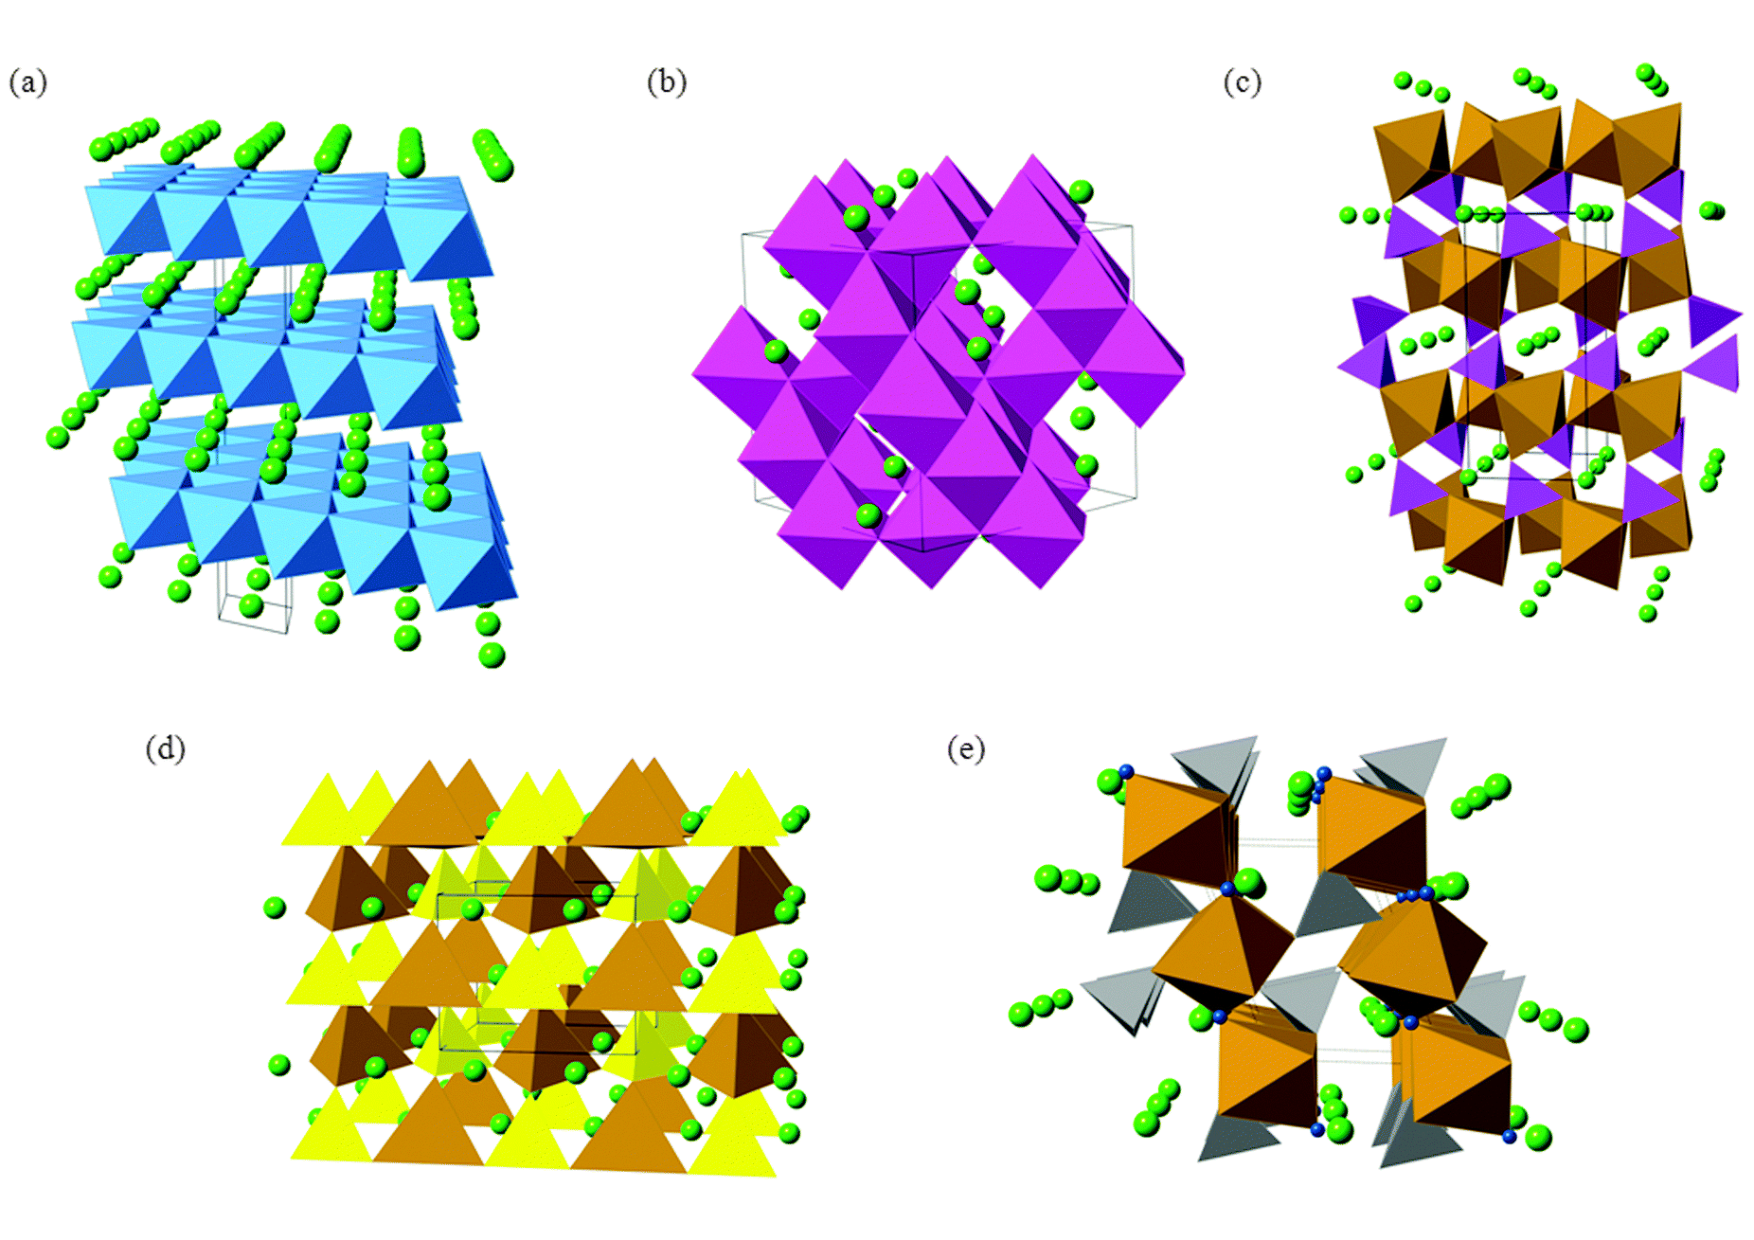
\includegraphics[scale=0.5]{figures/cathode_structures.pdf}
    \caption{Representative crystal structures of cathode materials for lithium-ion batteries: (a) layered $\alpha$-LiCoO$_2$; (b) cubic LiMn$_2$O$_4$ spinel; (c) olivine-structured LiFePO$_4$; (d) $\beta_{II}$-Li$_2$FeSiO$_4$; and (e) tavorite-type LiFeSO$_4$F. Li ions are shown as light green spheres, CoO$_6$ octahedra in blue; MnO$_6$ octahedra in mauve, Fe–O polyhedra in brown, PO$_4$ tetrahedra in purple, SiO$_4$ tetrahedra in yellow, SO$_4$ tetrahedra in grey, and in (e) fluoride ions in dark blue. Black lines demarcate one unit cell in each structure. Reproduced with permission from \citeauthor{islam2014lithium} \cite{islam2014lithium} - Published by The Royal Society of Chemistry.}
    \label{fig:cathode_structures}
\end{figure}

A large number of the most promising cathode materials for Li-ion batteries are transition metal (TM) oxides. These transition metal oxides most commonly adopt either a layered ($\alpha$-NaFeO$_2$) crystal structure or one derived from spinel-like (LT-LiCoO$_2$), however they can also take rock-salt form ($\alpha$-LiFeO$_2$), as presented in Figure \ref{fig:structure}. Some TM oxides are stable in various structural forms, such as lithium manganese oxide, which has been synthesised with layered, \cite{armstrong1996synthesis} spinel, \cite{mosbah1983phases} and rock-salt structures. \cite{dittrich1969kristallstruktur} For intercalation type cathodes used in Li-ion batteries, the structural framework is expected to remain relatively unchanged, with only small changes from lattice expansion/contraction. However, phase transitions can occur during the cycling process. For example, during cycling a phase transition can occur from the LiMn$_2$O$_4$ spinel structure to the LiMnO$_2$ rock-salt structure, partially due to the occurrence of oxygen evolution. \cite{peng2017atomistic} Phase transitions between layered and spinel structures are also widely observed. \cite{chen2018understanding} For example, \citeauthor{reed2001layered} investigated the layered to spinel phase transitions in Li$_x$MnO$_2$ using DFT modelling (cf. section~\ref{sec:dft}). \cite{reed2001layered} Their investigation determined that partially lithiated layered Li$_x$MnO$_2$ transitions to spinel in a two-stage process. Firstly, a large percent of Mn and Li ions quickly occupy tetrahedral sites, to form a meta-stable intermediate. Then, a more complex, coordinated, rearrangement of Mn and Li occurs to form spinel. Interestingly, this behaviour is in contrast to Li$_x$CoO$_2$ and understanding the reasons as to why, could prove useful for creating Mn-based cathode materials.

\begin{figure}
    \centering
    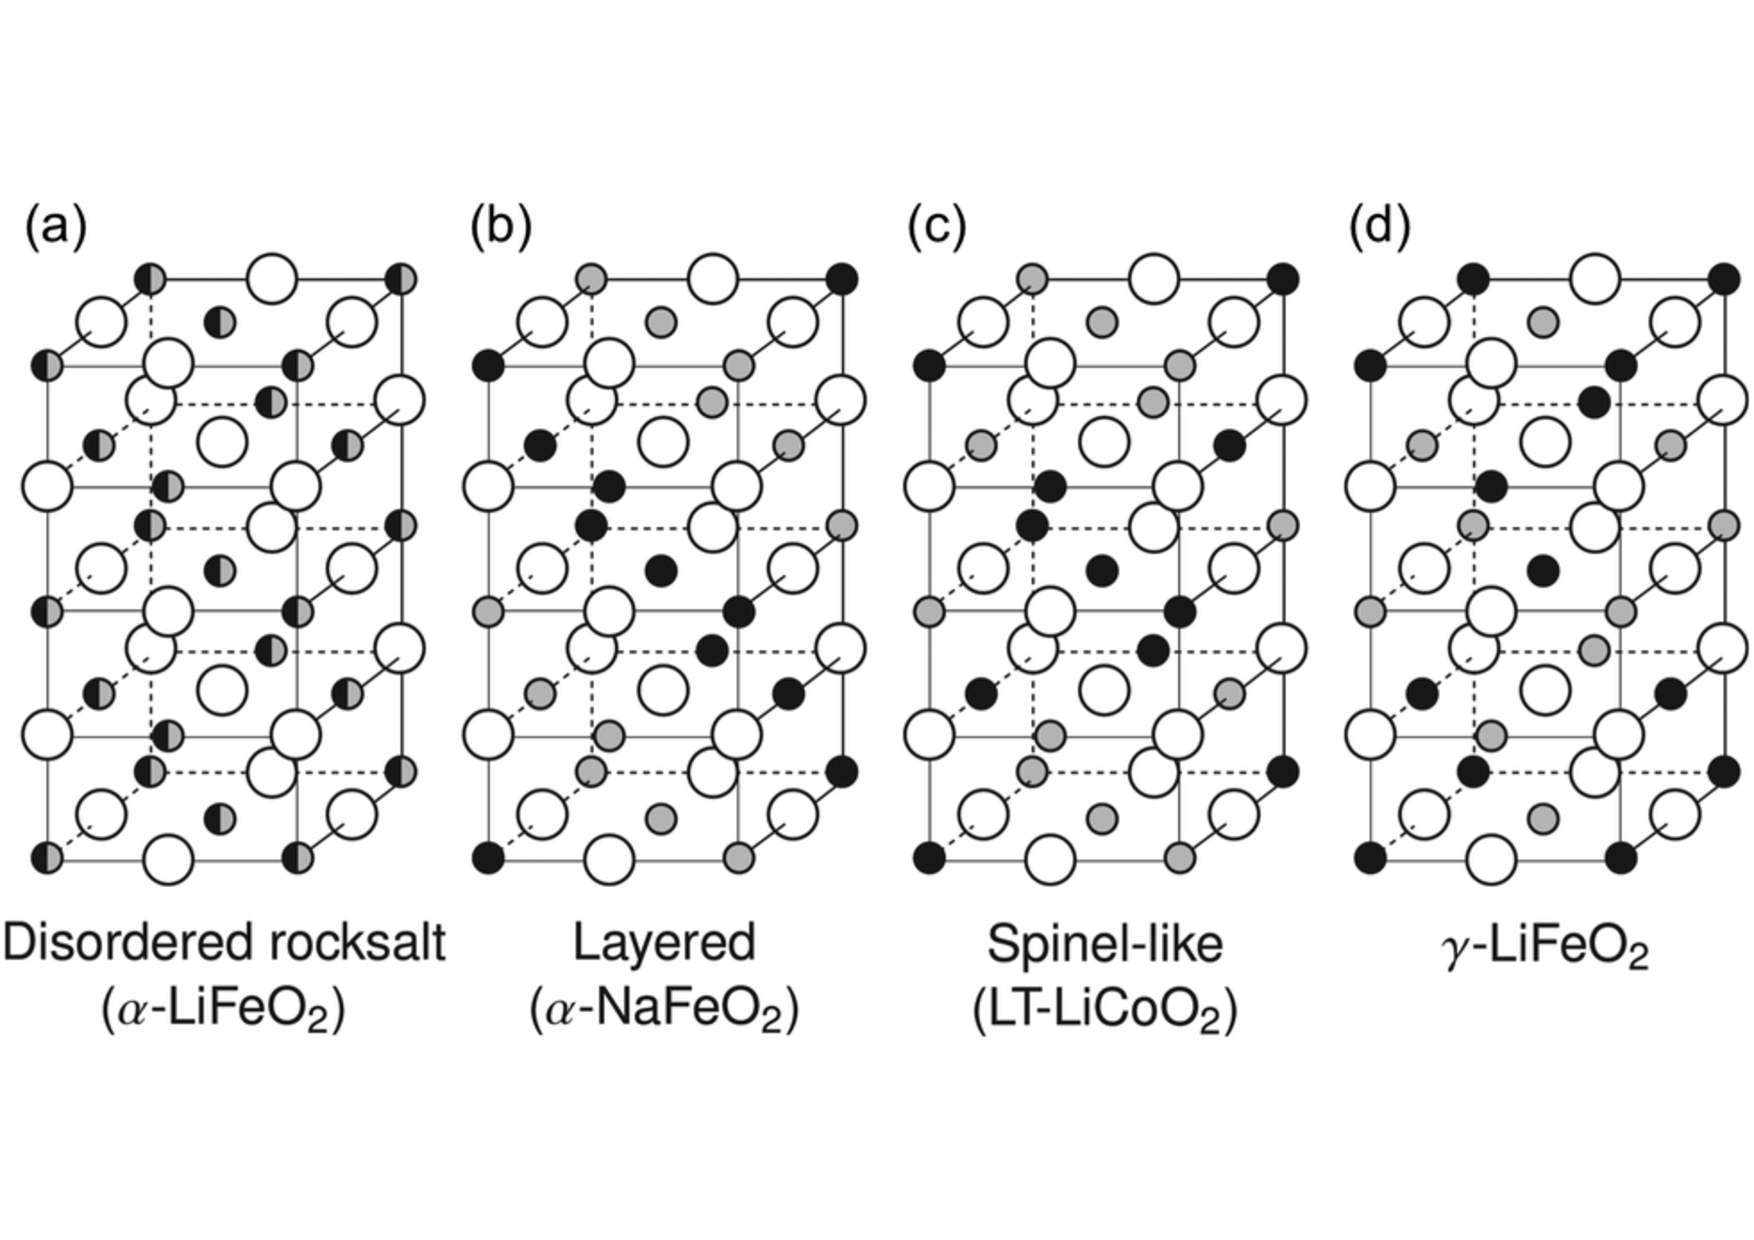
\includegraphics[scale=0.4]{figures/structures.pdf}
    \caption{Common rocksalt-type lithium transition metal oxide crystal structures: (a) the disordered rocksalt $\alpha$-LiFeO$_2$ structure in which all cation sites are equivalent, (b) the layered $\alpha$-NaFeO$_2$ structure, (c) the spinel-like low-temperature LiCoO$_2$ structure, (d) the $\gamma$-LiFeO$_2$ structure. Large empty circles indicate oxygen sites, small gray and black filled circles stand for lithium and transition metal sites, respectively. Reproduced with permission from \citeauthor{clement2020} \cite{clement2020} - Published by The Royal Society of Chemistry.}
    \label{fig:structure}
\end{figure}

\textbf{Micro-Structuring.} It is clear that control over bulk structure has an impact of the materials performance, as many properties are dependent on shape and size. \cite{bruce2008nanomaterials} The structural and micro-structural properties of a material are also vital to cycling stability of a cathode. For example, reducing the particle size of LiFePO$_4$ to the nano-metre scale is shown to increase the electrochemical performance, compared to the equivalent larger particles, by reducing transport path lengths. \cite{franger2006chemistry, ellis2007synthesis,malik2010particle} Selective structuring can also provide mechanical benefits, for example, where forces acting on the functional cathode during cycling, as the lattice expands and contracts with lithium intercalation, can cause plastic deformation and extinguish the desirable activities. \citeauthor{sayle2018stress} modelled diffusion-induced stress in layered-spinel Li-Mn-O composites, revealing structural resilience enabled by flexing of a porous structure. \cite{sayle2018stress} In this study \citeauthor{sayle2018stress} found the yield stress of the bulk material was 11.35 GPa, whilst the nanoporous material subjected to an equivalent strain experienced a stress of 4.32 GPa. In fact, it has been proposed that a $\beta$-MnO$_2$ host should be symmetrically porous and heavily twinned to maximise the cathode's electrochemical properties. \cite{sayle2009predicting} Further to this, intergrowing structures of two polymorphs of MnO$_2$, $\beta$-MnO$_2$ and R-MnO$_2$,\cite{Gupta2018} has shown to enhance cell performance,\cite{GUPTA2020227619} due to reduction in stresses and facile diffusion in more open structure of R-MnO$_2$.

% \textbf{Defects.} The micro-structure, such as the presence of grain-boundaries, stacking faults, and dislocations are essential to understanding the electrochemical behaviour and structural durability of cathode materials. \cite{sayle2006microstructure,sayle2009mechanical}. As defects form naturally in experiments and under ``real world'' battery use, their presence can have significant effects on the material properties, and therefore their role is important to understand. Knowledge of point defect types and their properties are widely investigated using atomistic modelling, more readily, using potential-based classical MD (cf. section~\ref{sec:molecular_dynamics}). Aspects such as the formation energetics of intrinsic atomic defects such as Schottky, Frenkel, and antisite disorder in a wide range of cathode materials have been investigated using MD using (in Kr\"{o}ger-Vink notation):

% \begin{equation}
%     \text{Li Frenkel: } \mathrm{Li}_{\mathrm{Li}}^{\times} \to \mathrm{Li}_{i}^{*}+V_{\mathrm{Li}}^{\prime}
% \end{equation}
% \begin{equation}
%     \mathrm{Li}_{2}\mathrm{O} \text{ Schottky-like: } 2 \mathrm{Li}_{\mathrm{Li}}^{\times}+\mathrm{O}_{\mathrm{o}}^{\times} \to 2 V_{\mathrm{Li}}^{\prime}+V_{\mathrm{O}}^{* *}+\mathrm{Li}_{2} \mathrm{O}
% \end{equation}
% \begin{equation}
%     \text{Antisite (cation exchange): } \mathrm{Li}_{\mathrm{Li}}^{\mathrm{x}}+\mathrm{M}_{\mathrm{M}}^{\times} \to \mathrm{Li}_{\mathrm{M}}^{\prime}+\mathrm{M}_{\mathrm{Li}}^{*}
% \end{equation}

% Within this notation, the subscript indicates the regular lattice or interstitial ($i$) positions and the superscript indicates the net charge, where $^{*}$ is positive and $^{\prime}$ is negative. $V$ in this case represents a vacancy and M is usually a transition metal. \citeauthor{islam2014lithium} summarises some of the most energetically favourable cathode materials in relation to the defects, investigated using potential-based techniques. \cite{islam2014lithium} NMC, LiMn$_2$O$_4$, and LiFePO$_4$ are among those reviewed by \citeauthor{islam2014lithium}. They find that the most favourable intrinsic defect in these materials are cation antisite defects, in which a small amount ($<3$\%) of metal ions (Fe$^{2+}$, Mn$^{2+}$, Ni$^{2+}$) occupy Li sites. The concentration of the defect is dependant on temperature and thus sensitive to the experimental synthesis conditions. In relation, \citeauthor{bruckner2014carbon}, using DFT, determined that there is a correlation between the oxygen vacancy defect concentration and voltage suppression for spinel LiNi$_{0.5}$Mn$_{1.5}$O$_4$. \cite{bruckner2014carbon}

% \citeauthor{gardiner2010anti} used the Mott-Littleton method, \cite{mott1938conducting} with a combined DFT and Classical MD study to look at defects and ion migration in LiFe$_{0.5}$Mn$_{0.5}$PO$_4$. \cite{gardiner2010anti} They showed that charge point defects form localised clusters, and can be studied through the calculation of binding energies. They determined that defect clustering can negatively impact the Li transport behaviour and can be identified as precursors to local ordering. 

% \textbf{Ion Doping.} In addition to intrinsic defect, atomistic methods can aid in investigating the effects of doping in cathode materials. These methods can provide estimations of the reaction energies for different dopant substitutions, and give insight into site-selectivity of dopants and trends in dopant solubility. For NMC materials, this is effectively LiCoO$_2$ doped with Ni and Mn. As previously mentioned, introducing Ni and Mn into the system increases the conductivity and electrochemical performance of the layered oxide, however ordering of these transition metals and their oxidation states within the NMC structure affects the cathode performance. This is discussed in more detail in Section \ref{sec:TM_ordering_NMC}.

% The electronic and magnetic features of the LiMn$_2$O$_4$ spinel framework are strongly dependent on doping in the cationic sublattice. For example, experimentally, \citeauthor{capsoni2002inhibition} determined that doping LiMn$_2$O$_4$ with as low as 1\% Ga${^3+}$ significantly modifies the temperature of the conductivity drop associated with Jahn-Teller (JT) distortion, preventing the transition observed near room temperature. \cite{capsoni2002inhibition} First principles using GGA/GGA+U (cf. section~\ref{sec:dft}), has also been employed to analyse the effect of doping LiMn$_2$O$_4$ on the JT distortion. In this study \citeauthor{singh2009suppression} found that doping with Cr and MG also suppressed the JT distortion, results of which were in good agreement with experiment. \cite{singh2009suppression} Doping of LiMn$_2$O$_4$ has also been shown to suppress some of the degradation mechanisms in the material. A joint experimental and computational study conducted by \citeauthor{zhang2016dual}, showed that dual-doping with Al/Co suppressed particle fracture during charge/discharge cycling. \cite{zhang2016dual} For the computational part of this study, \citeauthor{zhang2016dual} employed first principles calculations (DFT) of the undoped, Al and Co single-doped, and Al/Cl dual-doped LiMn$_2$O$_4$ to analyse the structural properties and differences. They found that although JT distortion of the Mn$^{3+}$O$_6$ octahedron is the origin of the lattice strain, the distribution of the mixed valence Mn ions is more prevalent at releasing lattice strain. The lattice mismatch on Li$^+$ intercalation and deintercalation was shown to be reduced in LiMn$_2$O$_4$ by dual doping with Al/Co, and reduce the volumetric shrinkage which occurs in cycling, which can account for the large reduction of cracks forming.

% Over the last decade, simulation studies have been conducted on a wide range of doped \ce{LiFePO4}, from monovalent to pentavalent cations. For monovalent cation doping \citeauthor{islam2005atomic} found that \ce{Na+} on \ce{Li+} sites showed low, favourable energies, \cite{islam2005atomic}, where \citeauthor{islam2005atomic} and \citeauthor{fisher2008lithium} found divalent doping with Zn/Cu/Mg on transition metal sites also gave low, favourable energies. \cite{islam2005atomic,fisher2008lithium} in contrast, supervalent doping of Ti$^{4+}$ and Nb$^{5+}$ on \ce{Li+} and Fe$^{2+}$ sites is energetically unfavourable. \cite{islam2005atomic} Co-doping with Si on P sites, and F on O sites, has also shown promising results, where there is an improvement in conductivity compared to undoped \ce{LiFePO4}. \cite{ban2012novel} \citeauthor{zhang2018first} used first principle calculations to conduction band structure calculations, analysing the formation energies, Debye temperature, and Poisson's ratios to determine that although the formation energy shows \ce{LiFePO4} is mechanically stable, doping the material can improve the mechanical stability. \cite{zhang2018first} Specifically, doping with Co can also enforce isotropic behaviour, as apposed to the anisotropic behaviour in \ce{LiFePO4}. This can help reduce the risk of microcracking and shear deformation of the material. A more recent study by \citeauthor{cholsuk2020first} used first principles methods (GGA+U) to investigate the effects of doping with Ti$^{4+}$ at Fe$^{2+}$ sites in lithium deficient environments, looking at the crystal and electronic structures, and the conductivity. \cite{cholsuk2020first} \citeauthor{cholsuk2020first} elucidates to the impurity states, and from use of climbing-image nudge elastic band (cNEB) calculations, they find that Li hopping can be promoted by doping with high Ti concentrations, enhancing the electronic and ionic conductivities.

\subsubsection{Ion Diffusion (Lucy)}
\label{sec:cathode_ion_diffusion}
As discussed in Section \ref{sec:diffusion}, diffusion coefficients can be calculated using multiple techniques, including ab-initio MD (DFT), Classical MD, and Monte Carlo. Diffusion coefficients, although important experimentally and for parameterising continuum models, are not the only diffusion property of interest on the atomistic scale. Properties such as diffusion mechanisms, hopping frequencies, and activation energy barriers are all vital to understanding Li-ion transport and charge/discharge rate behaviour. This is of particular interest for investigating the effects of grain-boundaries and interfaces on the migration routes and mechanisms. For example, in LiCoO$_2$ \citeauthor{moriwake2013first} determined that the activation energy, $E_a$, for Li migration \textit{along} a twin boundary is 0.20 eV, smaller than that in the bulk, while the $E_a$ \textit{across} a twin boundary is 0.4 eV. \cite{moriwake2013first}

The use of computational techniques can aid in providing information regarding a materials diffusion behaviour, which can not be fully understood experimentally. For example, \citeauthor{dixit2015classical} compared Li and Na diffusion in Li$_{0.25}$FePO$_4$ and Na$_{0.25}$FePO$_4$, respectively, by calculating the potential and free energy diffusion barriers and determining the nuclear quantum effects (NQEs) of the Li ions. \cite{dixit2015classical} Their calculations found that Li diffusion was faster than Na diffusion, which is in agreement with experiments. However, the authors also determined the NQEs for Li-ions were higher than for Na-ions and the quantum behaviour of the Li-ions was unusual. This information would not be possible to resolve using current experimental methods.

The cathode crystal structure is key to the available diffusion pathways in the material. First-principles calculations \cite{Morgan2004,ouyang2004first} and shell model simulations (MD)\cite{islam2005atomic} show Li$_x$FePO$_4$ is an olivine based structure which hosts Li over an interstitial network that has one-dimensional connectivity, i.e. 1-D diffusion, along the $b$ lattice vector of the orthorhombic cell.\cite{amin2006anisotropy} Li$_x$CoO$_2$ is a layered compound that accommodates Li ions within octahedral sites that form two-dimensional triangular lattices, i.e. 2-D diffusion, along the $b$ and $c$ lattice vector of the orthorhombic cell. \cite{van2000lithium} The spinel form of Li$_x$Mn$_2$O$_4$ has both tetrahedrally and octahedrally coordinated Li interstitial sites that form a three-dimensional network, i.e. 3-D diffusion, along all lattice vectors. \cite{thackeray1997manganese,proell20123d} Chemical diffusion coefficient of Li in an intercalation compound often has a strong dependence on Li concentration and crystal structure. The combination of first-principles cluster
expansion Hamiltonians with kinetic Monte Carlo simulations, as described in sections \ref{sec:cluster_expansion} and \ref{sec:monte_carlo} revealed that the Li diffusion coefficients of transition metal oxides (and sulfides) are very sensitive to the Li concentration and also to the degree of cation ordering. \cite{van2008nondilute,VanderVen2001, bhattacharya2011first,bhattacharya2010phase,VanDerVen2013} For example, \citeauthor{VanderVen2020} shows the calculated Li diffusion coefficients for the layered (2D) and spinel (3D) forms of Li$_x$TiS$_2$ as a function of Li concentration. \cite{VanderVen2020,VanDerVen2013,van2008nondilute,bhattacharya2011first} This is presented in Figure \ref{fig:LixTiS2_diffusion} along with the structural images and vacancy mechanisms highlighted. Here it can be seen that not only are there orders of magnitude differences in the Li diffusion coefficients, but the shape of the diffusion/Li concentration relation is very different. This shows how the crystal structure, and thus the active diffusion pathways, play a crucial role in determining the concentration dependence of the diffusion coefficients in these materials.

\begin{figure}
    \centering
    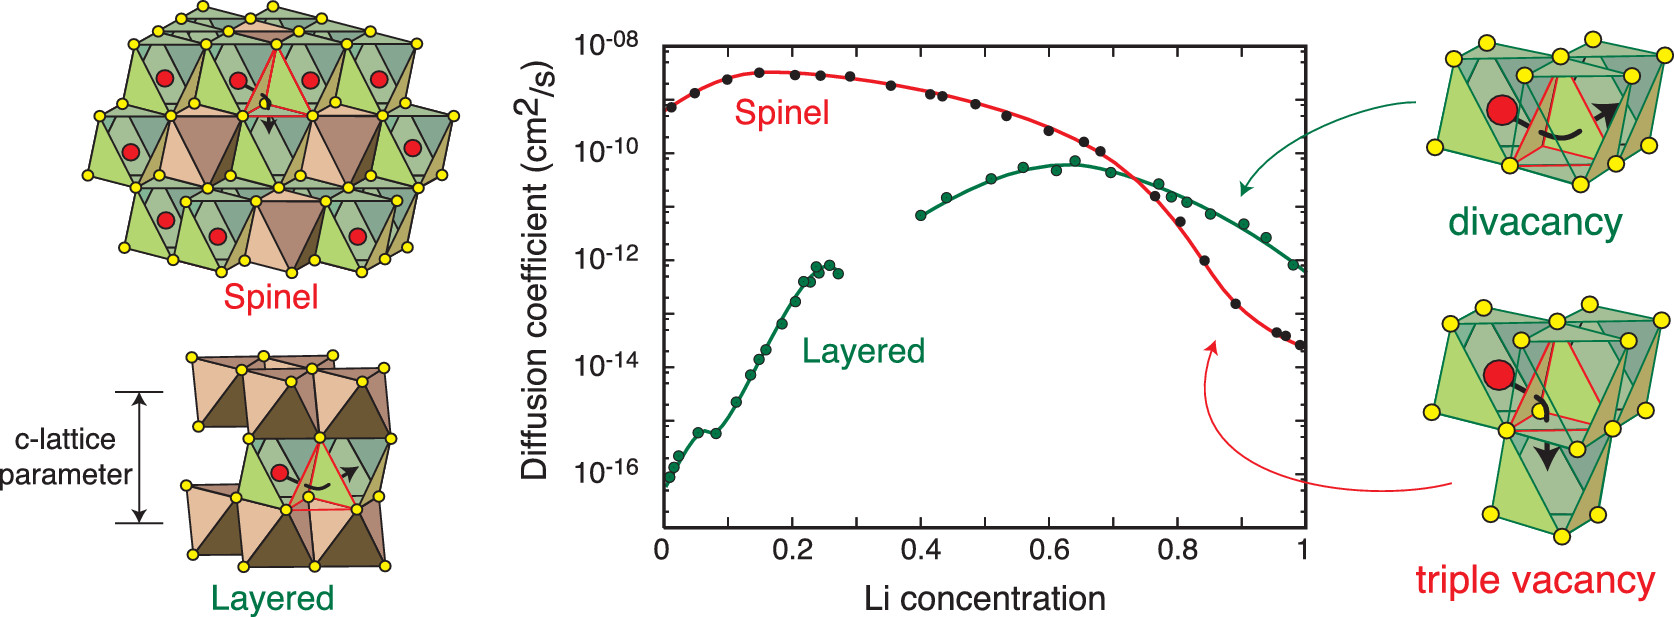
\includegraphics[scale=0.26]{figures/LixTiS2_diffusion.jpeg}
    \caption{ Chemical diffusion coefficient of Li in an intercalation compound often has a strong dependence on Li concentration and crystal structure. Reproduced with permission from \citenum{VanderVen2020} - Adapted from \citenum{VanDerVen2013} - Copyright 2013 American Chemical Society.}
    \label{fig:LixTiS2_diffusion}
\end{figure}

When discussing the conductivities and the rates at which a battery can be charged and discharged, we must consider the ion diffusion pathways, the activation energies, and migration mechanisms which govern the Li transport. These details can often be challenging to determine solely through experimental studies. Atomistic modelling has a proven record to aid in this investigation through calculations of migration energy barriers and identifying diffusion pathways and their dimensionality, as discussed above. We have already eluded that diffusion is sensitive to the Li concentration, however, the exact relation is through the activation barriers. Early DFT studies \cite{van2000lithium,van2001lithium} of Li$_x$CoO$_2$ systems showed that the lithium diffusion was predominately through a divacancy mechanism, when $0\leq x < 1$. At infinite vacancy dilutions however diffusion is through a single vacancy mechanism. \cite{islam2014lithium} There are two hopping mechanisms at play here; oxygen dumbbell hops and tetrahedral site hops. Oxygen dumbbell hopping occurs when there is a single vacancy and a lithium has to travel between two occupied adjacent lithium sites to reach the vacant lithium site. Tetrahedral site hopping occurs when there are divacant or trivacant sites i.e.  when one or both of the adjacent lithium sites are vacant. \cite{van2001lithium} Oxygen dumbbell hopping has a significantly lower migration barrier energy compared to tetrahedral site hopping, which highlights the sensitivity of the activation barrier to the lithium concentration. Experimental studies of mixed-TM layered oxides, such as Li(Ni$_{0.5}$Mn$_{0.5}$)O$_2$, have reported site exchange between Li and Ni ($\sim$ 8-12 \%). \cite{choi2005structural} DFT has been used to aid in understanding the effects of this on the lithium mobility. \cite{kang2006electrodes,laubach2009structure} (De)intercalation of lithium in the material changes the distances between the layers. As Li is removed from the structure, there is a reduced ``barrier'' between the oxygen layers which start to repel one another. By calculating the activation energy as as a function of the distance between the O layers on either side of the Li layers, a trend between increased distance O layer distance and lower activation energy is seen. \cite{kang2006electrodes,laubach2009structure}

In addition to the crystal structure and available diffusion pathways, doping the cathode material can also influence the material properties, including ion diffusion. NMC cathodes are effectively LiCoO$_2$ doped with Ni and Mn. As previously mentioned in section \ref{sec:cathode_intro}, introducing Ni and Mn into the system, forming a mixed-TM layered oxide, increases the diffusion/conductivity and electrochemical performance. Detailed computational studies of mixed-TM oxides have been scares due to their complexities. An illustration of this is the complexities which arise from transition metals, such as Fe, Ni, Co, and Mn, which exhibit localised oxidation states. This can be further complicated, or influenced by TM ordering. For instance, \citeauthor{lee2013solid} investigated the effects of TM disorder on the electrochemical properties of Li$_x$Ni$_{0.5}$Mn$_{1.5}$O$_4$ using cluster expansion and Monte Carlo methods (cf. sections~\ref{sec:cluster_expansion} and \ref{sec:monte_carlo}). The authors determined a correlation between Li vacancy ordering and TM ordering. \cite{lee2013solid} \citeauthor{hao2016quaternary} found similar evidence for Li$_x$(Mn$_y$Ni$_{1-y}$)$_2$O$_4$. \cite{hao2016quaternary} These also have an effect on the diffusion properties of the material. TM ordering in NMC cathodes is discussed in more detail in section \ref{sec:TM_ordering_NMC}. Using experimental techniques \citeauthor{capsoni2002inhibition} found that doping the cationic sublattice of spinel LiMn$_2$O$_4$ with as low as 1\% Ga${^3+}$ significantly modifies the temperature of the conductivity drop associated with Jahn-Teller (JT) distortion, preventing the transition observed near room temperature. \cite{capsoni2002inhibition} This allows for a wider temperature window for the higher conductivity phase. First principles using GGA/GGA+U (cf. section~\ref{sec:dft}), was also employed to analyse the effect of doping LiMn$_2$O$_4$ on the JT distortion. In this study \citeauthor{singh2009suppression} found that doping with Cr and MG also suppressed the JT distortion, and thus the associated temperature of the conductivity drop. \cite{singh2009suppression} 

\subsubsection{Redox and Electronic Properties (Ryan)}
The cathode operates by the deintercalation of Li$^+$ on charging, and the reinsertion of Li$^+$ on discharging. The charge is balanced by the oxidation and reduction of the transition metal ion, e.g. LiCo$^{3+}$O$_2$ $\rightleftharpoons$ Li$_{1-x}$Co$^{4+}$O$_2$ + $x$Li$^+$ + $x$e$^-$. 

The specific capacity of most LIB cathode materials is limited by the number of electrons per transition metal cation that can participate in the redox reaction. However, the recent discovery of oxygen redox reactivity, O$^{2-}$ $\to$ (O$_2$)$^{n-}$,  in Li-excess cathode materials\cite{Koga2013, Sathiya2013, Oishi2015, Sathiya2015, McCalla2015, Cao2015, Shimoda2016, Chen2016, Luo2016a, Hy2016, Muhammad2016, Seo2016, Gent2017, Zhan2017,  Zheng2017,Assat2018, BenYahia2019, naylor2019depth, Hua2019, House2020, Li2019, Eum2020, Gent2020, Sharpe2020} has prompted further investigation.

DFT has been pivotal in shedding light on this phenomenon, in conjunction with a range of experimental techniques. This technique can be used to analyse the atomic charge and electronic structure of each ground state, enabling the charge compensation during delithiation to be correctly attributed during simulated charging. For example, \citeauthor{Xiao2012} used DFT to calculate the oxygen charge compensation in Li$_2$MnO$_3$.\cite{Xiao2012} Likewise, other authors have done the same with Li$_2$IrO$_3$,\cite{Li2019} Li$_5$FeO$_4$,\cite{Zhan2017} and Li[Li$_{0.25}$Ni$_{0.20}$Mn$_{0.55}$]O$_{1.93}$.\cite{Shimoda2016} \citeauthor{Yao2018} were able to propose a sequence of redox events for delithiation of Li$_4$Mn$_2$O$_5$;\cite{Yao2018} first, cationic redox, Mn$^{3+}$/Mn$^{4+}$, dominates for Li$_x$Mn$_2$O$_5$, when 4 $\geq$ x $>$ 2. Then anionic redox, O$^{2-}$/O$^{1-}$, dominates for Li$_x$Mn$_2$O$_5$, when 2 $\geq$ x $>$ 1. Finally, mixed cationic (Mn$^{4+}$/Mn$^{5+}$) and anionic (O$^{2-}$/O$^{1-}$) redox for Li$_x$Mn$_2$O$_5$, when 1 $\geq$ x $\geq$ 0. Meanwhile, fluorinated materials such as Li$_2$Mn$_{2/3}$Nb$_{1/3}$O$_2$F\cite{Lee2018} and Li$_2$MnO$_2$F\cite{Sharpe2020} were found to exhibit some overlap between the redox processes, suggesting that the substitution of O by F favours lower Mn oxidation states, therefore leading to more redox overlap with oxygen. DFT has also been used to establish the band structure for cathode materials, determining which transition metal orbitals hybridise more with the O(2p) orbitals\cite{Cao2015, Sathiya2013a} and to identify hole states.\cite{Zhan2017, Xiao2012}

\citeauthor{Sathiya2013a} highlighted the importance of the M-(O$_2$) covalency in ensuring that the anionic redox is reversible and to prevent the release of O$_2$ gas from the structure at high states of charge.\cite{Sathiya2013a,Saubanere2016} Further work by these authors combined transmission electron microscopy (TEM), neutron diffraction and ab-initio studies to visualise the (O-O)$^{n-}$ peroxo-like dimer in Li-rich Li$_2$Ir$_{1-x}$Sn$_x$O$_3$, postulating that it may be responsible for the improved capacity observed.\cite{McCalla2015} In a combined experimental and computational study, \citeauthor{Gent2017} observed a strong correlation between anion redox, cation migration and open-circuit voltage hysteresis in Li-rich layered oxides.\cite{Gent2017} \citeauthor{Hong2019} offered an explanation for the strong coupling between anion redox and structural disordering in Li rich layered oxides; they found local stabilisation of short $\sim$1.8 \AA \ metal-oxygen $\pi$ bonds and $\sim$1.4 \AA \ O-O dimers during oxygen redox.\cite{Hong2019} The formation of this species necessitated the decoordination of oxygen to a single covalent bond through formation of vacancies at neighbouring cation sites, driving cation disorder.

\citeauthor{Seo2016} showed that anion redox chemistry is heavily dependent on the anion nearest-neighbour coordination environment.\cite{Seo2016} In particular, they described how more Li-O-Li configurations lead to more potentially labile oxygen electrons, which led to greater O redox chemistry. A DFT study of Li$_5$FeO$_4$ found that O oxidation only occurred on those O anions coordinated to six Li cations, and not those coordinated to at least one Fe (e.g. OLi$_5$Fe).\cite{Zhan2017} A similar result was found with Li$_2$MnO$_2$F; those oxygens coordinated to at least five Li (e.g. OLi$_5$Mn) in the fully lithiated state were the first to oxidise, whereas those coordinated to three or fewer (e.g. OLi$_3$Mn$_3$) did not undergo oxidation at all. This showcased a more continuous variation in the O-redox potential, dependent on the number of Li coordinated to a given O$^{2-}$ ion.\cite{Sharpe2020} Recent computational screening work on layered oxide cathodes using hybrid DFT has reported trends in O-redox activity associated with the electrostatic (Madelung) energy at oxygen sites.\cite{Davies2020}

\citeauthor{Chen2016} investigated delithiation and kinetic processes in Li$_2$MnO$_3$ using hybrid DFT, and found that Li extraction is charge-compensated by oxidation of the oxide anion, so that the overall delithiation reaction involves lattice oxygen loss.\cite{Chen2016} Localised holes on oxygen (O$^-$) are formed at the first step, but due to their instability, lead to oxygen dimers (O-O is approximately 1.3 \AA) and eventually to the formation of molecular O$_2$. This then facilitates Mn migration to the octahedral site in the vacant Li layer, leading to a spinel-like structure. The authors proposed that, in order to make use of the oxide anion as a reversible redox centre, it is essential to stabilise the O$^-$ hole species and prevent oxygen dimerization. This should then prevent Mn migration, O$_2$ evolution and structural transformation. DFT has also been used to show the formation of O$_2$ at high states of charge in Li$_2$MnO$_2$F\cite{Sharpe2020} and Li$_{1.2}$Ni$_{0.13}$Co$_{0.13}$Mn$_{0.54}$O$_2$, \cite{House2020a} agreeing with experimental RIXS data, and to report superoxide formation in Li$_2$VO$_2$F, in agreement with EPR studies.\cite{Chang2020}

\subsubsection{Transition Metal Ordering in NMC Layered Oxides (Lucy)}
\label{sec:TM_ordering_NMC}
Cation/anion ordering also plays a vital role in the properties/activity of a material, such as the physical and electrochemical properties. A topical illustration of this is the NMC cathode materials, where recent experimental studies show that spin interaction of the transition metal ions is a major challenge. \cite{duan2019insights, xiao2018insight} The varying compositions, charge distributions, and electronegativities of the transition metals lead to a mixture of valence states, where Ni can exist as Ni$^{2+}$, Ni$^{3+}$, and Ni$^{4+}$, Co can exist as Co$^{3+}$ and Co$^{4+}$, and Mn exists as Mn$^{4+}$. \cite{xiao2018insight} The interactions between these mixed valence states poses a challenge to identifying ground states. As NMC materials, such as NMC811, emerge as front runners for commercialisation, research into their specific chemistry has become of great interest. Recently, several computational studies have been performed to analyse the influence of transition metal valence states on the stability and structure-property relationships of NMC materials. \cite{sun2017electronic,dixit2017origin, hoang2016defect,dixit2017unraveling} \citeauthor{sun2017electronic} analysed five NMC compositions, observing that random arrangement of transition metals present similar thermodynamic states, which is in contract with experiment identifying that transition metal spin interactions vary the stability of any NMC composition. \cite{sun2017electronic}  Recently, a study by \citeauthor{rana} analysed the transition metal oxidation states in NMC811, using HSE06 DFT. Here, the authors highlight the difficulties in assigning oxidation states using various techniques, and determine that the lowest energy structures for pristine NMC811 contain a mixture of Ni$^{2+}$ and Ni$^{3+}$, giving a composition of \{1Ni$^{2+}$;7Ni$^{3+}$;1Mn$^{4+}$;1Co$^{3+}$\}. \cite{rana} The complex nature of the transition metal oxidation states limited this study to the pristine NMC811 material, and is currently being expanded to delithiated states.

\subsubsection{Vibrational and Thermal Properties (Hui)}
An important contribution to the thermodynamic properties at finite temperature is the vibrational partition function, which can be evaluated by calculating the material’s normal modes of lattice vibrations. A number of researchers have theoretically addressed the vibrational contribution to the material thermodynamic properties in LIBs, especially in NMC cathodes. \cite{du2016insight,yang2019highly,yang2020chemical} There are several works studying on cathode materials beyond NMC. \citeauthor{shang2012lattice} employed first-principles phonon calculations with a mixed-space approach to probe the lattice dynamics and finite-temperature thermodynamic properties of olivine structure \ce{LiMPO4} (M = Mo, Fe, Co, Ni).\cite{shang2012lattice} They reported that \ce{LiMPO4} from Mn, Fe, Co, to Ni have increase trend for zero-point vibrational energy while decrease trend for vibrational contribution to Gibbs energy due to the decreasing phonon densities of state at the low frequency region of \ce{LiMPO4}.
Very recent, lattice dynamics study has been expand to solid electrolytes , which probably aids the discovery of lithium fast-ion conductors. \cite{sagotra2019influence} 

Computing lattice thermal conductivity have been developed by two major approaches, namely  solving Boltzmann transport equation (BTE) using anharmonic lattice dynamics and molecular dynamics (MD) simulations. \citeauthor{puligheddu2019computational} compared lattice thermal conductivity values from these two methods and found a satisfactory agreement.\cite{puligheddu2019computational} The comparison used empirical potentials and took account the effects of fourth order phonon scattering, temperature-dependent phonon frequencies and reported the effects difference between quantum and classical statistics.

Using BTE within the relaxation-time approximation, \citeauthor{mattila2020lattice} reported the highly anisotropic lattice thermal conductivities in isotopic \ce{LiCoO2}, close to the values in \citeauthor{yang2019highly}'s work\cite{yang2019highly,yang2020chemical}, and illustrated the effect of the alkali metal atom by replacing Li by Na.\cite{mattila2020lattice} They found explained by significantly shorter phonon lifetimes in \ce{LiCoO2}. They found that in-plane lattice thermal conductivities in \ce{NaCoO2} is $\sim$0.7 time larger than that in \ce{LiCoO2} at room temperature since the former has significantly larger phonon life timers. While \citeauthor{feng2020quantum} report much lower thermal conductivity values by including four-phonon scattering, though a different functional, the local density approximation (LDA), was used for exchange and correlation.\cite{feng2020quantum} They also investigated the thermal transport reduction during delithiation (charging) due to reduced phonon velocities and increasing anharmonicity. Furthermore, grain-boundary effect reduced thermal transport and  suppressed thermal conducivites in polycrystals are well reproduced when grain sizes were reduced down to several nm in either BTE or MD simulations. \cite{he2019thermal}

Besides, the thermal conductivity investigation can be also performed on anode and many more compounds.\cite{qian2016anisotropic, wei2018tunable} Very recently, a high-throughput study has been reported for 37 binary rocksalt and zinc blende material systems, in which the authors highlight the importance of high-order phonon-phonon interactions based on harmonic calculations. \cite{xia2020high}

\subsection{Surfaces (Lucy)}
Surface structures and morphologies of cathode particles is difficult to determine using experimental methods alone, which is where computation investigations can provide vital insight, resulting in the growing field of nanoionics. \cite{zhang2013nanomaterials} More specifically, atomistic modelling is ideally suited in terms of time- and length- scales to directly compare to experimental measurements. \cite{catlow2010modelling} As previously discussed in Section \ref{sec:methods}, under \ref{sec:molecular_dynamics}, there are benefits to using both DFT and Classical MD, with the main trade of between accuracy and time- and length- scales. Despite the differences between the two techniques, they are often complementary and in good agreement. Both DFT and classical MD have been extensively used to investigate the surfaces and morphologies of layered oxides, spinel oxides, and olivine phosphates, which will be briefly discussed here. These techniques have also be used to investigate cathode materials in sodium-ion batteries, which is covered in more detail in Ref.~\citenum{islam2014lithium}.

With oxides at the forefront of the battery revolution, it is unsurprising there have been many DFT and classical MD studies into layered LiCoO$_2$, LiMn$_2$O$_4$ spinel, MnO$_2$-type and related materials, looking at properties including the surfaces, nanostructures, and morphologies.\cite{kramer2009tailoring,xu2011identifying, daheron2009surface,kim2012first,benedek2011simulation,karim2013surface,leung2012first, tompsett2013nanostructuring} Surface energies for low-index layered LiCoO$_2$ surfaces, as a function of external Li and O chemical potentials, revealed the (0001) and (10\={1}4) surfaces were present for all reasonable values of Li and O chemical potentials, whereas the (01\={1}2) surface was only stable under oxidising conditions. \cite{kramer2009tailoring} While studies into the low-index surface facets of LiMn$_2$O$_4$, (100),(110), and (111) determine the (111) surface to be the most stable through site exchange of under-coordinated Mn on the surface, exhibiting a cubo-octahedral type predominately comprising \{111\} surfaces. \cite{karim2013surface} Other studies show the Mn-terminated (111) surfaces undergoing surface reconstruction, and indicating the Li-terminated (001) surface having the lowest energy. \cite{benedek2011simulation}

It has also been shown electronic spin state transitions occur on the surfaces of stoichiometric LiCoO$_2$. Here \citeauthor{qian2012electronic} found that the trivalent Co ions at the surface adopt an intermediate spin state if they are square–pyramidal coordinated and a high spin state if they are pseudo-tetrahedral coordinated. This highlighted that low-coordinated geometries on the particle surface effect the Co$^{3+}$–Co$^{4+}$ redox potential. \cite{qian2012electronic} \citeauthor{hong2019electronic} investigated the surface properties of LiCoO$_2$ nanoplatelets and their chemical modifications with Al$^{3+}$, using combined experimental and theoretical approaches.\cite{hong2019electronic} Their models also showed the electronic structures of several LiCoO$_2$ surface facets are different from those of the bulk, attributing this to the altered spin states of surface Co$^{3+}$ atoms. The authors found splitting of the Co 3d–O 2p states, which were linked with high-spin-state Co$^{3+}$ at the surface. Partial substitution of Co$^{3+}$ by Al$^{3+}$ was found to increase the ratio of low-spin-state Co$^{3+}$ at the surface, resulting in a distinct change in the intensity ratio of the split Co 3d–O 2p states. 

When exposed to certain environmental conditions LiCoO$_2$ releases Co cations, a known toxicant. \citeauthor{abbaspour2020dft} has applied DFT (with different functionals) and thermodynamics modelling to study the LiCoO$_2$ surface transformations. \cite{abbaspour2020dft} They assessed how the calculated predictions for ion release depend on aspects of the structural surface model. Here, the authors propose a generalised scheme for predicting a threshold pH at which Co release becomes favourable, providing information that could be used to inform macroscopic contaminant fate models. More recently, these authors have furthered this investigation in cation dissolution at the LiCoO$_2$ surface, finding that at pH of 7 16 \% of surface Co undergoes dissolution. \cite{abbaspour2020dft}

The surface structures of LiFePO$_4$ exhibit a complex and uneven topology due to the size difference of Li$^+$, Fe$^{2+}$, and PO$_{4}^{3-}$. The majority of terminating surfaces undergo fairly considerable relaxation, which makes predictions based on rigid terminations unreliable. Although LiFePO$_4$ can be synthesised in multiple morphologies, \cite{chen2006electron,ellis2007synthesis} exposing different surfaces, studies on the (010) surfaces are particularly interesting. This surface is normal to the most facile pathway for lithium ion conduction, \cite{islam2010recent} reducing the diffusion path lengths for lithium at the surface, enhancing the electrochemical performance of the cathode. \textit{First-principles} calculation of the diffusion pattern and energy landscape of lithium in LiFePO$_4$ showed the energy barrier for the Li diffusion along (010) is lower than the other directions, i.e. (100), indicating that the Li diffusion in LiFePO$_4$ is one dimensional. \cite{tankhilsaikhan2019density} Understanding processes such as the lithium (de)intercalation on the LiFePO$_4$ (010) surface is important for developing effective approaches to further improve the material's rate performance. Using DFT calculations, \citeauthor{xu2019insight} find the extraction of Li from the surface layer has a significant effect on the work function of LiFePO$_4$ (010) surface, which provides evidence for whether Li atoms are present in the outermost layer of LiFePO$_4$ (010) surface or not. \cite{xu2019insight} Here, the authors also calculate the redox potential and formation energies for extracting Li from different (010) surface layers. They find that extracting lithium from the outer surface layers has the lowest redox potential and formation energy, indicating that it is energetically favorable to extract Li first from the surface layer. \citeauthor{xu2019insight} propose a new method that surface work functions can be used for providing insight into the lithium (de)intercalation on the LiFePO$_4$ (010) surface. \cite{xu2019insight}

\citeauthor{zhang2020observation} used a combined experimental and computational (DFT) approach to investigate the preferential cation doping on the surface of LiFePO$_4$ and its effect on properties. \cite{zhang2020observation} The authors found that for all chosen dopants there was increased ratios of Fe$^{3+}$/Fe$^{2+}$ oxidation on the particle surfaces, while the core atoms remained closer to that of the pristine undoped material. This indicates the dopants are predominantly pushed to the particle surfaces during phase formation. This disparity in distribution of dopant across the core and surface results in improved conductivities. \cite{zhang2020observation} \textit{ab initio} MD simulations with XRD and microscopy experiments on the LiFePO$_4$ cathode show Li-ions migrating along the surface facilitated by solvent molecules. \cite{li2018fluid} This work establishes fluid-enhanced surface diffusion as a key factor in tuning phase transformation in aniostropic solids.

\subsection{Interfaces (Arihant)}
\label{sec:cathode_interfaces}
Although the cathode-electrolyte interface (CEI) is thinner than the SEI at the anode, it is still quite complex in structure and composition.\cite{Gauthier2015, Edstrom2004} DFT based simulations can provide insight into adsorption trends,\cite{Bhandari2020} reaction pathways and energetics,\cite{Tebbe2015a, Tebbe2015b} and migration barriers for Li-ion transfer.\cite{Bhandari2019} etc. The electrolyte in a Li-ion battery is typically a Li salt, for example LiPF$_6$ in an organic carbonate solvent, such as ethylene carbonate (EC), propylene carbonate (PC), diethyl carbonate (DEC) or dimethyl carbonate (DMC). The LiPF$_6$ electrolyte reacts with trace amounts of moisture to form HF,\cite{Tebbe2015a} which is highly corrosive and reacts with the cathode surface to form fluoride-based products.\cite{Tebbe2015b} The organic carbonate solvent  also react with the cathode surface to form a series of decomposition products.\cite{Tebbe2016} The adsorption of organic carbonate and fluoride-based products is the first step in the series of reactions that lead to the formation of CEI. The decomposition reaction of cyclic organic carbonates proceeds via ring opening. The reaction of ring opening of cyclic organic carbonates has an energy barrier which is predicted to be around 0.62 eV on (100) LiMn$_2$O$_4$ surfaces,\cite{leung2012first} over 1 eV on (101$\Bar{4}$) LiCoO$_2$ surfaces,\cite{Tebbe2016} and around 0.29 eV on (101$\Bar{4}$) Li(Ni,Mn,Co)O$_2$ surfaces,\cite{Xu2017} via the DFT-NEB method (sec. \ref{sec:dft}, \ref{sec:methods_neb}).\cite{JONSSON1998} While experimental studies on composition of CEI have shown presence of both solvent-decomposition and fluoride-based products on most oxide cathodes, such as LiMn$_2$O$_4$, LiNiO$_2$ LiCoO$_2$ and LiNi$_{0.8}$Co$_{0.2}$O$_2$, no solvent reaction or solvent decomposition products are detected on LiFePO$_4$.\cite{Edstrom2004, Malmgren2010} Recent calculations of adsorption energies based on DFT have shown that adsorption preference of HF over EC leads to the entire LiFePO$_4$ nano-particle being covered by fluoride based products, which further leads to their dominant presence in the CEI.\cite{Bhandari2020} Based on DFT simulations, it is also possible to design suitable coatings in order to prevent cathode degradation,\cite{Tebbe2015b} These calculations can shortlist effective candidate materials for experiments and guide experiments. Thus the atomistic methods not only provide the necessary insights needed in order to rationalise the experimental observations but novel solutions to mitigate cathode degradation.

Apart from the complexity of structure of the CEI, another challenge is to understand the Li-ion migration mechanism at the CEI, which impacts the The rate capability of Li-ion batteries. The Li-ion conductivity in the bulk of electrolytes is around 1 S/cm (cf. sec. \ref{sec:electrolytes}) which is several orders of magnitude higher than that in the electrode materials (cf. sections~\ref{sec:anodes_ion_diffusion} and \ref{sec:cathode_ion_diffusion}) (around 10$^{-7}$-10$^{-2}$ S/cm).\cite{park2010review, VanDerVen2013} However, the complex structure of the CEI and unknown mechanism of Li-ion transfer across it has hindered the understanding of the kinetics at the interface. Recent DFT-NEB calculations on LiFePO$_4$ cathode have estimated an energy barrier of 756 meV for Li to move from a near-surface solvated cluster to a sub-surface vacancy in the LiFePO$_4$ cathode material.\cite{Bhandari2019} Due to preferential adsorption of fluoride on LiFePO$_4$ surfaces,\cite{Edstrom2004, Bhandari2020} the energy barrier has been found to decrease to 410 meV in presence of fluoride. Nevertheless, the interfacial energy barrier is higher than that in the bulk cathode material, which is estimated to be around 270-290 meV.\cite{Morgan2004,Dathar2011} This highlights a rate-limiting behaviour of the interface in the overall Li-ion diffusion process in Li-ion batteries. This study motivates further such investigation on other cathode electrolyte interfaces, especially with the recently developed advanced-methods for characterising the interface as described in sec. \ref{sec:dft+cont}.  

\subsection{Outlook and challenges for cathodes (Lucy/Ryan)}
%NMC materials and Li-rich
Lowering the cost, increasing capacity, and improving the sustainability of battery materials is becoming more critical as we move towards large-scale deployment of lithium-ion batteries for applications such as electric vehicles. \cite{dunn2011electrical} Here, we highlight some of the outstanding challenges for cathodes and how atomistic modelling can aid in gaining insight and work towards solving them.

Ni-rich NMC layered oxides are favorite candidates for cathode materials due to their high gravimetric and volumetric energy densities.\cite{li2020high} However, Ni-rich NMC materials have three critical challenges: cycle instability, thermal instability, and air instability. These are all linked with the instability of Ni$^{3+}$ and Ni$^{4+}$ at the surface/interface. Other cathode materials, such as oxyfluorides, have worked towards solving some of these issues, however, there are still outstanding challenges for the surface and interfaces for which atomistic modelling is vital:
\begin{itemize}
    \item In Ni-rich NMC the unstable Ni$^{3+}$ and Ni$^{4+}$ react aggressively with the electrolyte to form thick cathode-electrolyte interphase (CEI) layers and cause Ni and Mn dissolution. The dissolute transition metals then migrate to the anode and limit the battery cyclability, \cite{li2017dynamic,li2018mn} which in turn causes electrolyte decomposition, leading to thick anode-electrolyte interphase (SEI) layers forming. Understanding and preventing CEI and SEI formation is a crucial challenge for improvement of both conventional and solid-state batteries. Atomistic modelling plays a key role in this. Although electrochemical spectroscopic techniques have been used to obtain molecular scale information, further detail is needed in order to obtain more reliable information. This may not be resolvable using current experimental techniques, which is where atomistic modelling can provide the fundamental understanding needed guide experimental studies.
    \item Phase transitions at the surface of cathode materials occur at a high-state-of-charge and affect the surface reactivity, resulting in increased TM dissolution and CEI/SEI formation. The effect of this is rapid capacity fading during cycling. \cite{li2019comprehensive} Co-free Li-rich layered oxides, such as Li[Li$_{0.2}$Mn$_{0.6}$Ni$_{0.2}$]O$_{2}$, are appealing due to their low cost and high capacities (300 mAh g$^{-1}$). \cite{kim2004electrochemical,armstrong2006demonstrating} However, these materials undergo layered to spinel transitions due to low octahedral site stability of Mn$^{3+}$ which leads to voltage decay during cycling and Mn dissolution,\cite{MnDissolution2016} making these materials challenging to employ as a practical cathode. Atomistic insight into the mechanisms involved in these phase transitions, gained through \textit{ab initio} and classical MD methods, can provide essential detail and understanding needed to prevent these phase transitions occurring.
    % O redox & O2 formation rewrite
    \item Some cathode materials show reversible O-redox, with lower voltage hysteresis and, in the case of O$_2$ formation, reincorporation into the lattice.\cite{Sharpe2020} On the other hand, other materials show irreversible O-redox, with O$_2$ lost from the surface, \cite{Nakayama2020, Chen2016, House2020a} which leads to unwanted side reactions with the electrolyte. The formation and potential loss of molecular O$_2$ is likely to be heavily dependent on local structure. In the case of Li$_2$MnO$_2F$, DFT showed that O$_2$ is formed only in O-Li rich areas, not in O-Mn rich areas.\cite{Sharpe2020} Meanwhile, other oxyfluorides such as Li$_2$VO$_2$F, don’t show molecular O$_2$ formation at all, but instead form superoxides on charging.\cite{Chang2020} Use of DFT allows examination of the local structure in much greater detail than can be achieved experimentally, providing essential insight to this problem.
\end{itemize}

It is challenging to model disordered systems, as by their very nature, they can have an almost infinite arrangement of atoms. Use of computational techniques, such as cluster expansion, to generate low-energy structures of disordered rock-salts is a promising route to more realistic DFT studies.\cite{Lun2020}

%Interatomic potentials
As discussed in section~\ref{sec:potential_fitting}, fitting interatomic potentials of a system is key to improving the quality of research conducted through classical modelling. It is commonplace to reuse potentials from literature sources, without determining how they were fitted, which can lead to inaccuracies in the calculations performed. For example, if a potential for a cathode material was fitted only to lattice parameters, elastic constants, and the bulk modulus, then it would not be accurately representative of the cathode redox properties. If properties such as the dielectric constant were included, then redox chemistry would be better represented. In effect, interatomic potentials in literature are not necessarily transferable to different types of study. It is not feasible to fit to every material property, however, a broader range of properties, most relevant to the study being conducted is required. There are tools in development \cite{gale_empirical_1996,Stukowski_2017,wen_kim-compliant_2017, Morgan2020BuckFit} which are making this potential fitting process more accessible to atomistic modellers, with the ability to fit to a larger range of parameters, however, there is still a need for improved transparency in the publication of studies using interatomic potentials. Use of machine learning to develop potentials has also shown to be a promising avenue. \citeauthor{deringer2019machine} recently published a progress update, showing how machine learning is improving interatomic potentials by ``learning'' from electronic-structure data, giving increased accuracy in approximating material properties. \cite{deringer2019machine}

%concluding statement
In-depth insight into the elemental distribution, electronic structure, and crystalline structure under electrochemical conditions is challenging to achieve experimentally. Atomistic techniques, including DFT and MD, are well suited to providing the insight needed for these properties. However, future research and development of cathode materials will require collaborative efforts, involving the disciplines of chemistry, physics, material science, nanoscience/nanotechnology, and computational modelling/simulation.\cite{yu2018electrode}
\end{document}